\documentclass[12pt, titlepage]{article}

\usepackage{fullpage}
\usepackage{array}
\usepackage{longtable}
\usepackage{pdfpages}
\input{../../Common.text}

\title{Interview Report for \progname{}}
\author{\authname}
\date{\today}

\begin{document}

\pagenumbering{gobble}
\maketitle
\pagenumbering{roman}
\tableofcontents
\newpage
\pagenumbering{arabic}

\section{Introduction}

Spectropica is a customizable educational game suite designed to support autistic learners through interactive learning activities. Care Team Members (CTMs), including parents, caregivers, and educators, can personalize activities according to individual learning needs and review learner progress.

To gather stakeholder feedback and inform the development of Spectropica, the team conducted \textbf{four stakeholder interviews and one additional email exchange with a special education teacher}. The email format was used because a suitable time for a live interview could not be scheduled.

The participants represented educational, caregiving, parental, and developmental psychology perspectives. Their feedback provided insight into the challenges autistic children may experience during educational activities, the limitations of existing learning tools, and the features that could make Spectropica more accessible and useful.

This report documents the interview methodology, questions, participant responses, and analysis of the findings. It also identifies how the feedback can inform Spectropica's requirements, design decisions, and future evaluation.

\section{Purpose and Goals}

The purpose of the interviews was to better understand the needs of Spectropica's intended users and the individuals who support their learning.

The interviews focused on six goals:
\begin{enumerate}
\item \textbf{Learning needs and challenges:} Identify difficulties children experience when using educational games and completing learning activities.
\item \textbf{Accessibility and engagement:} Understand sensory preferences, sources of frustration, and strategies that support engagement.
\item \textbf{Personalization:} Determine which game settings, instructions, and activities would be most valuable to customize.
\item \textbf{Progress tracking:} Identify useful measures of learning progress and information CTMs would want recorded.
\item \textbf{Existing tools and limitations:} Understand what works well in current educational games and where improvements are needed.
\item \textbf{Success criteria:} Identify outcomes that stakeholders would consider meaningful evidence of Spectropica's usefulness.
\end{enumerate}

The goal was not to assume that all autistic learners have the same needs, but to identify common considerations while recognizing differences between individual children.

\section{Methodology}

\subsection{Participants}

Five stakeholders contributed to the report through four interviews and one email exchange.

\begin{longtable}{|p{0.08\textwidth}|p{0.52\textwidth}|p{0.26\textwidth}|}
\hline
\textbf{ID} & \textbf{Stakeholder} & \textbf{Method} \\ \hline
\endfirsthead
\hline \textbf{ID} & \textbf{Stakeholder} & \textbf{Method} \\ \hline
\endhead
P1 & Special education teacher, Senior Kindergarten to approximately Grades 3--4 & Email questionnaire \\ \hline
P2 & Educational assistant with early childhood education experience & Interview responses \\ \hline
P3 & Developmental psychology expert and project supervisor & Interview responses \\ \hline
P4 & Care Team Member & Interview responses \\ \hline
P5 & Parent of an autistic child & Interview responses \\ \hline
\end{longtable}

Participant identifiers are used throughout the report to avoid including personal names or identifying information.

The participants provide different perspectives on educational games. P1 and P2 describe professional classroom experiences, P3 provides developmental psychology and design guidance, and P4 and P5 describe caregiving and family experiences.

\subsection{Data Collection}

The team used open-ended questions covering technology proficiency, learning difficulties, accessibility, rewards, personalization, progress tracking, and existing educational games.

The special education teacher provided written responses by email because a live interview could not be arranged. The educational assistant, CTM, parent, and our project supervisor provided responses through interviews conducted between November 2nd, 2026 to November 17, 2026.

The educational assistant, Care Team Member, and parent interviews were
conducted in person.

The questions allowed participants to describe their own observations and experiences. Some participants answered related questions together or did not provide a response to every question. These gaps are preserved rather than replaced with assumed answers.

\subsection{Data Analysis}

Responses were reviewed and organized into themes corresponding to the interview goals. Similar observations were compared across participants, while differences were retained to avoid presenting individual experiences as universal.

Each theme was considered in relation to Spectropica's design, including learner interactions, personalization, game sessions, rewards, and the CTM dashboard.

The findings below distinguish between stakeholder observations and proposed development implications. Suggested changes are not automatically treated as approved requirements.

\section{Interview Questions}
\label{sec:interview-questions}

The main questionnaire is listed below. Wording varied slightly between
interviews, and the developmental psychology interview used a separate
discussion agenda.

\begin{enumerate}
\item What is your level of comfort/proficiency with technology such as
  browsers, iPads, and tablet apps?
\item What level of comfort/proficiency with technology, specifically
  educational games, do you observe in children learning at a Grades 3--5 level?
  \begin{enumerate}
  \item What parts do they struggle with?
  \item What parts do they excel in?
  \item What aspects of games aggravate or frustrate them?
  \item Have you observed any differences in how autistic children interact
    with these technologies?
  \end{enumerate}
\item What do the children you work with generally struggle with when it comes
  to learning?
\item Based on your experience, are there any learning needs or challenges you
  have observed more frequently among autistic children? How do these vary
  between individual children?
\item What tools or techniques help?
\item What types of rewards or reinforcement have you found effective for
  children generally? Have you noticed differences in how individual autistic
  children respond?
\item What circumstances aggravate them?
\item What is hard to do on your own or outside your control but would help?
\item When a child becomes frustrated or disengaged during a learning activity,
  what strategies do you use to help them?
\item Are there particular visual, auditory, or interactive features in
  educational games that children find overwhelming or distracting?
\item What accommodations or accessibility features have you found most
  effective when supporting autistic children during digital learning
  activities?
\item What aspects of an educational game would be most valuable to customize,
  such as difficulty, visuals, sounds, instructions, or activity duration?
\item How do you measure their progress in learning?
\item What is hard to track manually but would be helpful to have documented
  over time?
\item What indicators tell you that a child is improving at a particular skill?
\item What information would you want an educational game to record
  automatically?
\item What educational games or learning tools do you currently use with
  children, and what features do you find most helpful?
\item When children use educational games, how much assistance do they
  typically need from an adult? Are there particular tasks they struggle to
  complete independently?
\item What would make a progress dashboard easy or difficult for you to
  interpret?
\item What are the biggest limitations of the current games that exist?
\item If you were to use an educational game like Spectropica with a child,
  what improvements or outcomes would make you consider it successful?
\end{enumerate}

The full available source responses are retained in the \hyperref[app:interview-responses]{appendices}.

\section{Findings and Analysis}

\subsection{Learning Challenges and Instructions}

A recurring finding was that familiarity with technology does not necessarily mean a child can independently understand or complete an educational activity.

P1 reported that younger students often struggle with reading instructions, logging in, and navigating unfamiliar menus. However, they can become very comfortable with familiar games and remember how they work.

P2 similarly explained that many children, including autistic children, are proficient with technology. Difficulties are often related to understanding the activity rather than operating the device. Some students benefit from simplified instructions, examples, or having instructions read aloud.

P4 observed that children may delete games they do not understand, despite being comfortable with typical interface elements such as buttons, icons, and typing. P5 emphasized the importance of highly guided learning activities and gradually introducing unfamiliar concepts.

\noindent\textbf{Analysis:} These findings suggest that Spectropica should distinguish between a learner's ability to operate a device and their ability to understand an educational task. An interface can be technically simple while still presenting instructions or learning objectives that are too difficult.

\noindent\textbf{Development implications:} The team should review the clarity of instructions, availability of audio guidance, replayable instructions, and the use of examples before activities. Navigation should remain predictable, and learners should not need to understand complex menus to begin playing.

\subsection{Sensory Accessibility and Frustration}

All four education and caregiving participants identified sensory or environmental distractions as factors that can interfere with learning.

P1 identified loud sounds, busy screens, moving objects, and excessive buttons as potential distractions. P2 described auditory overload and frustration when children cannot pause or retry an activity.

P4 reported that excessive background visuals, repetitive sounds, and visually locked content can distract from the task. However, P4 also noted that repetition can support engagement and learning.

P5 similarly identified background conversations, movement, and other environmental distractions. At the same time, P5 described insufficient stimulation as a limitation of some existing games.

P3's meeting notes discussed reducing distractions during learning tasks, allowing sound to be switched off, and using high contrast when presenting problems.

\noindent\textbf{Analysis:} The responses do not support a single ideal stimulation level. Some learners may find animation or sound distracting, while others may benefit from or enjoy these elements. The important finding is the need for flexibility.

\noindent\textbf{Development implications:} Spectropica should support configurable sensory settings, particularly audio and visual stimulation. The team should also review pause and retry functionality and consider whether distracting elements can be reduced during learning tasks without removing engaging elements entirely.

\subsection{Personalization and Individual Learning Needs}

Personalization was one of the strongest recurring themes.

P1 prioritized adjustable difficulty, sound, activity duration, and familiar images. P2 emphasized difficulty levels and instructions, while also supporting customization of activity duration and presentation.

P4 highlighted activity duration, hint wording, reward access, and stimulation levels. P5 emphasized different auditory voices, visual themes, and gradual increases in difficulty.

P3's interview notes also supported allowing learners to adjust stimulation and content, alongside greater CTM access to game settings.

\noindent\textbf{Analysis:} The participants agreed on the importance of personalization but prioritized different settings. This reinforces the need to design for individual learners rather than relying on a fixed configuration.

There is also a distinction between \textbf{CTM-controlled settings} and \textbf{learner-controlled settings}. CTMs may need to establish appropriate educational content and difficulty, while learners may benefit from independently adjusting sensory preferences.

\noindent\textbf{Development implications:} The Game Personalization and Template modules should be reviewed to ensure the relevant settings can be configured without excessive effort. The team should clarify which settings learners can change themselves and which require CTM permissions.

\subsection{Rewards, Motivation, and Engagement}

Participants described different ways of encouraging children to participate in learning activities.

P1 identified praise and opportunities to choose the next activity, while noting that some children prefer quiet acknowledgment rather than large celebrations.

P2 described varying verbal encouragement and offering activities connected to a child's interests.

P4 mentioned encouragement, periodic rewards, cosmetic items, and access to preferred activities. P5 described how preferred rewards changed over time, from tangible rewards and activities to verbal praise and celebrations.

P3's notes suggested providing rewards after questions while varying the rewards rather than repeating the same response.

\noindent\textbf{Analysis:} The responses suggest that rewards may support engagement, but their effectiveness depends on the learner. A reward that motivates one child may be distracting or uninteresting to another.

P5 also emphasized that learning unfamiliar concepts can require connecting them to familiar, preferred activities.

\noindent\textbf{Development implications:} The Rewards and Cosmetics module should be reviewed for customizable reinforcement and appropriate variation. Reward presentation should account for sensory preferences, and the educational objective should remain clear rather than allowing rewards to overshadow learning.

\subsection{Managing Frustration and Disengagement}

Participants described strategies that reduce frustration without forcing children to continue an activity.

P1 suggested offering breaks, checking whether instructions were understood, or returning to an easier step.

P2 emphasized gradually introducing activities, allowing breaks, and avoiding excessive instructions.

P4 described calming the situation, offering hints, providing short breaks, and using verbal encouragement. P5 emphasized communicating when an activity would end and explaining what enjoyable activity could follow.

\noindent\textbf{Analysis:} These responses highlight the importance of learner control and predictable activity structure. Frustration may arise from task difficulty, unclear expectations, or an activity continuing longer than the learner expects.

\noindent\textbf{Development implications:} The team should review whether activities can be paused, restarted, or exited appropriately. Configurable duration, clear activity expectations, and accessible hints could help CTMs adapt activities to individual attention spans.

\subsection{Progress Tracking and Learning Outcomes}

The interviews revealed that stakeholders evaluate learning progress using more than correct answers.

P1 considers how much assistance a child requires, whether they remember a skill later, and whether they can apply it outside the game.

P2 uses observations and Individual Education Plans (IEPs). The participant also identified response time, required guidance, and optional notes as useful indicators.

P4 described vocabulary recall, mathematical proficiency, engagement, problem-solving speed, and the ability to connect previously learned concepts. The participant also wanted to record repeated successful completions, time between attempts, and common mistakes.

P5 emphasized applying learned vocabulary and skills in everyday contexts, along with tracking changes in cooperation, social skills, and willingness to accept new activities.

\noindent\textbf{Analysis:} A central finding is that completing an activity correctly does not necessarily demonstrate independent understanding or skill retention.

The participants identified two categories of information:
\begin{itemize}
\item \textbf{Automatically observable gameplay data:} Attempts, accuracy, response times, hints, completed difficulty levels, and repeated successes.
\item \textbf{Contextual observations:} Adult assistance, behavior outside the application, skill generalization, and changes in willingness to participate.
\end{itemize}

Spectropica can record the first category directly, but the second requires human observation or input.

\noindent\textbf{Development implications:} The Game Session, Database, and Dashboard modules should distinguish automatically collected data from manually recorded observations. Optional CTM notes may provide context that gameplay metrics alone cannot capture.

\subsection{Dashboard Preferences}

Participants wanted progress information to be understandable, although their preferred presentation differed.

P1 preferred clear labels and simple trends rather than excessive graphs or scores without context.

P2 suggested limiting the amount of information shown at once and using checkmarks or numerical progress levels.

P4 preferred line graphs, bar graphs, contrasting colours, tooltips, and straightforward data export.

P5 suggested separating progress by skill, showing percentages and levels, and allowing different chart formats and date selections.

\noindent\textbf{Analysis:} These preferences demonstrate that a single dashboard layout may not meet every CTM's needs. However, all participants emphasized understanding progress without unnecessary difficulty.

\noindent\textbf{Development implications:} Spectropica should prioritize a clear dashboard overview while considering options for more detailed information, charts, and exported records. Dashboard labels should communicate what each metric measures and avoid presenting gameplay results as broader developmental assessments.

\subsection{Existing Educational Games and Their Limitations}

Participants identified several existing tools and limitations.

P1 described matching games, sequencing activities, and digital books, while emphasizing the value of quick setup and adjustable difficulty.

P2 highlighted communication applications and fine-motor activities. The participant also raised concerns about distracting features, time constraints, and excessive engagement with games.

P4 identified Otismo, Cubic Frog, and Talking Tom/Angela/Ben. The participant considered insufficient customization, unclear instructions, and unsatisfying rewards important limitations.

P5 identified Cubic Frog and Proloquo2Go. The participant described activities that begin at an inappropriate difficulty level, use overly complex vocabulary, or provide insufficient stimulation.

\noindent\textbf{Analysis:} The main opportunity identified by the interviews is not simply creating another educational game. It is providing educational activities that can be adapted to individual learning needs while giving CTMs useful information about performance.

P3's notes similarly emphasized identifying a meaningful gap in existing games designed for autistic learners.

\noindent\textbf{Development implications:} The team should use these findings to evaluate Spectropica's personalization, instructional design, reward system, and progress-reporting features against the limitations stakeholders described.

\subsection{Stakeholder Definitions of Success}

Participants described success in terms of learning, independence, and practical usefulness.

P1 emphasized engagement, decreasing assistance, and applying skills outside the game.

P2 wanted the game to support independent practice and classroom learning without replacing conventional education.

P4 prioritized progressively meeting learning objectives, visualizing progress, sharing information between CTMs, and adjusting settings when a learner becomes uncomfortable or disengaged.

P5 wanted the system to help CTMs identify suitable learning goals, recommend appropriate activities, and track progress toward those goals.

\noindent\textbf{Analysis:} These responses suggest that successful gameplay alone is not sufficient to demonstrate Spectropica's educational value. The game must also support meaningful learning objectives and provide useful information to CTMs.

P5's request for developmental-level evaluation represents a stakeholder need for better guidance. It should not be interpreted as evidence that Spectropica can clinically assess a child's developmental level.

\noindent\textbf{Development implications:} The team should evaluate whether CTMs can configure appropriate activities, understand recorded progress, and adjust future activities based on that information.

\subsection{Classroom and Family Perspectives}

The classroom participants (P1 and P2) and the family and care-team
participants (P4 and P5) agreed that children need guidance when an activity
is unfamiliar and that difficulty and sensory settings should reflect
individual needs. Both groups described distractions that can interfere with
learning, including distracting sounds or movement.

P1 and P2 emphasized what helps a child get started and practise in the
classroom, including clear instructions, examples, and manageable steps.
P4 and P5 emphasized how CTMs can adapt an activity over time, including
changing hints, sounds, or difficulty and using progress data to guide
future choices. The groups also differed in their dashboard preferences.
P1 and P2 favoured simple summaries, while P4 and P5 described ways to
explore progress in more detail, such as charts or skill breakdowns.

These perspectives suggest keeping instructions and dashboard summaries
easy to scan while making personalization and detailed progress views
available to CTMs when they need them.

\section{Development Implications and Traceability}
\label{sec:development-traceability}

The following table connects the interview findings to potential design actions and observable outcomes for future evaluation. These are \textbf{recommendations for review}, not claims that requirements have already been implemented or approved. Participant IDs link to their appendix records. Question numbers refer to Section~\ref{sec:interview-questions} and guide readers to the corresponding questionnaire topics.

\begin{longtable}{|p{0.23\textwidth}|p{0.15\textwidth}|p{0.22\textwidth}|p{0.28\textwidth}|}
\hline
\textbf{Interview evidence} & \textbf{Relevant area} & \textbf{Proposed development action} & \textbf{How we'll evaluate it} \\ \hline
\endfirsthead
\hline \textbf{Interview evidence} & \textbf{Relevant area} & \textbf{Proposed development action} & \textbf{How we'll evaluate it} \\ \hline
\endhead
\hyperref[app:participant-1]{P1}, \hyperref[app:participant-2]{P2}, \hyperref[app:participant-4]{P4}, \hyperref[app:participant-5]{P5}: Difficulty understanding tasks\par {\small Q2--Q5} & Game Session & Provide clear instructions, examples, and accessible assistance & Offer clear instructions and a worked example. Observe whether the learner starts the first task and record any adult prompts needed. \\ \hline
\hyperref[app:participant-1]{P1}, \hyperref[app:participant-2]{P2}, \hyperref[app:participant-3]{P3}, \hyperref[app:participant-4]{P4}, \hyperref[app:participant-5]{P5}: Different sensory preferences\par {\small Q10--Q12} & Game Personalization & Support adjustable audio and visual stimulation & Check whether a CTM can adjust sound and visuals and whether the activity reflects the selected settings. \\ \hline
\hyperref[app:participant-1]{P1}, \hyperref[app:participant-2]{P2}, \hyperref[app:participant-4]{P4}, \hyperref[app:participant-5]{P5}: Individual learning needs\par {\small Q12} & Game Personalization, Template & Support difficulty, duration, and instruction customization & Ask a CTM to configure an activity for a sample learner. Verify that difficulty, duration, and instructions match their choices. \\ \hline
\hyperref[app:participant-1]{P1}, \hyperref[app:participant-2]{P2}, \hyperref[app:participant-3]{P3}, \hyperref[app:participant-4]{P4}, \hyperref[app:participant-5]{P5}: Different reward preferences\par {\small Q6} & Rewards and Cosmetics & Support appropriate, varied reinforcement & Observe how learners respond to different reward options and record which options they choose when offered a choice. \\ \hline
\hyperref[app:participant-1]{P1}, \hyperref[app:participant-2]{P2}, \hyperref[app:participant-4]{P4}, \hyperref[app:participant-5]{P5}: Frustration and disengagement\par {\small Q7, Q9, Q11--Q12} & Game Session & Review pause, retry, hints, and activity duration & Check whether a learner can pause, resume, retry, or request a hint when they get stuck. \\ \hline
\hyperref[app:participant-1]{P1}, \hyperref[app:participant-2]{P2}, \hyperref[app:participant-4]{P4}, \hyperref[app:participant-5]{P5}: Need for meaningful progress data\par {\small Q13--Q16} & Game Session, Database & Record attempts, hints, performance, and completion & Check the recorded results against a sample session. Ask a CTM to identify a recurring mistake and choose a follow-up activity. \\ \hline
\hyperref[app:participant-1]{P1}, \hyperref[app:participant-2]{P2}: Value of contextual observations\par {\small Q13--Q16} & Dashboard, Database & Consider optional CTM notes & Ask a CTM to add and retrieve a note for a session, then explain how it helps them interpret the result. \\ \hline
\hyperref[app:participant-1]{P1}, \hyperref[app:participant-2]{P2}, \hyperref[app:participant-4]{P4}, \hyperref[app:participant-5]{P5}: Dashboard usability\par {\small Q19} & Dashboard, Charting & Provide understandable summaries and relevant detail & Ask a CTM to find a skill trend and explain what it shows without help. \\ \hline
\hyperref[app:participant-4]{P4}: Sharing progress between CTMs\par {\small Q21} & Care Team, File Import/Export & Review authorized sharing and export workflows & Verify that an authorized CTM can share or export the intended information and that an unauthorized CTM cannot. \\ \hline
\hyperref[app:participant-3]{P3}: Curriculum and game-design guidance\par {\small meeting notes} & Game Suite, Game Session & Review curriculum alignment and the educational purpose of game activities & Check whether each task in a sample activity gives learners practice with its stated curriculum objective. \\ \hline
\end{longtable}

These findings provide evidence for reviewing the project's existing requirements and identifying areas where clarification or changes may be appropriate.

\section{Limitations}

The findings are based on a small group of stakeholders and should not be treated as representative of all autistic learners.

Participants described their own experiences, and some responses differed substantially. The special education teacher's experience includes younger students, while Spectropica's intended learning level is approximately Grades 3--5. The interviews also did not involve direct evaluation of a completed Spectropica application.

The developmental psychology interview was documented through meeting notes rather than a verbatim transcript. These notes provide useful design guidance but should not be presented as direct quotations.

No autistic learner was directly interviewed in the available materials. The feedback therefore represents professional, caregiving, and parental perspectives rather than direct learner testimony.

\section{Conclusion}

The four interviews and additional email exchange provided several perspectives on the needs of autistic learners and the individuals supporting them.

The strongest recurring findings were the importance of individualized learning activities, adjustable sensory settings, clear instructions, flexible rewards, and meaningful progress tracking.

The participants also highlighted that educational progress cannot be evaluated solely through accuracy or completed activities. Information about assistance, engagement, and the application of skills outside the game may be important when interpreting learner performance.

These findings will inform the team's review of Spectropica's personalization, gameplay, reward, and reporting features. They also provide a basis for developing future evaluation activities focused on whether CTMs can effectively configure games and interpret learner progress.

\appendix
\section{Interview Transcripts and Email Exchange}
\label{app:interview-responses}

This appendix organizes the interview and email records by participant.

\subsection{Email Exchange with the Special Education Teacher (P1)}
\label{app:participant-1}

\noindent\textbf{Collection method:} Email correspondence.

\noindent\textbf{Participant:} Special education teacher working with students from Senior Kindergarten through approximately Grades 3--4.

The teacher was unable to schedule a live interview, so the team collected
responses through email. The following pages reproduce the original email
exchange, including the questionnaire and responses.

The participant addressed all 21 questionnaire topics, including navigation difficulties, sensory preferences, instructional support, rewards, progress tracking, and educational outcomes.

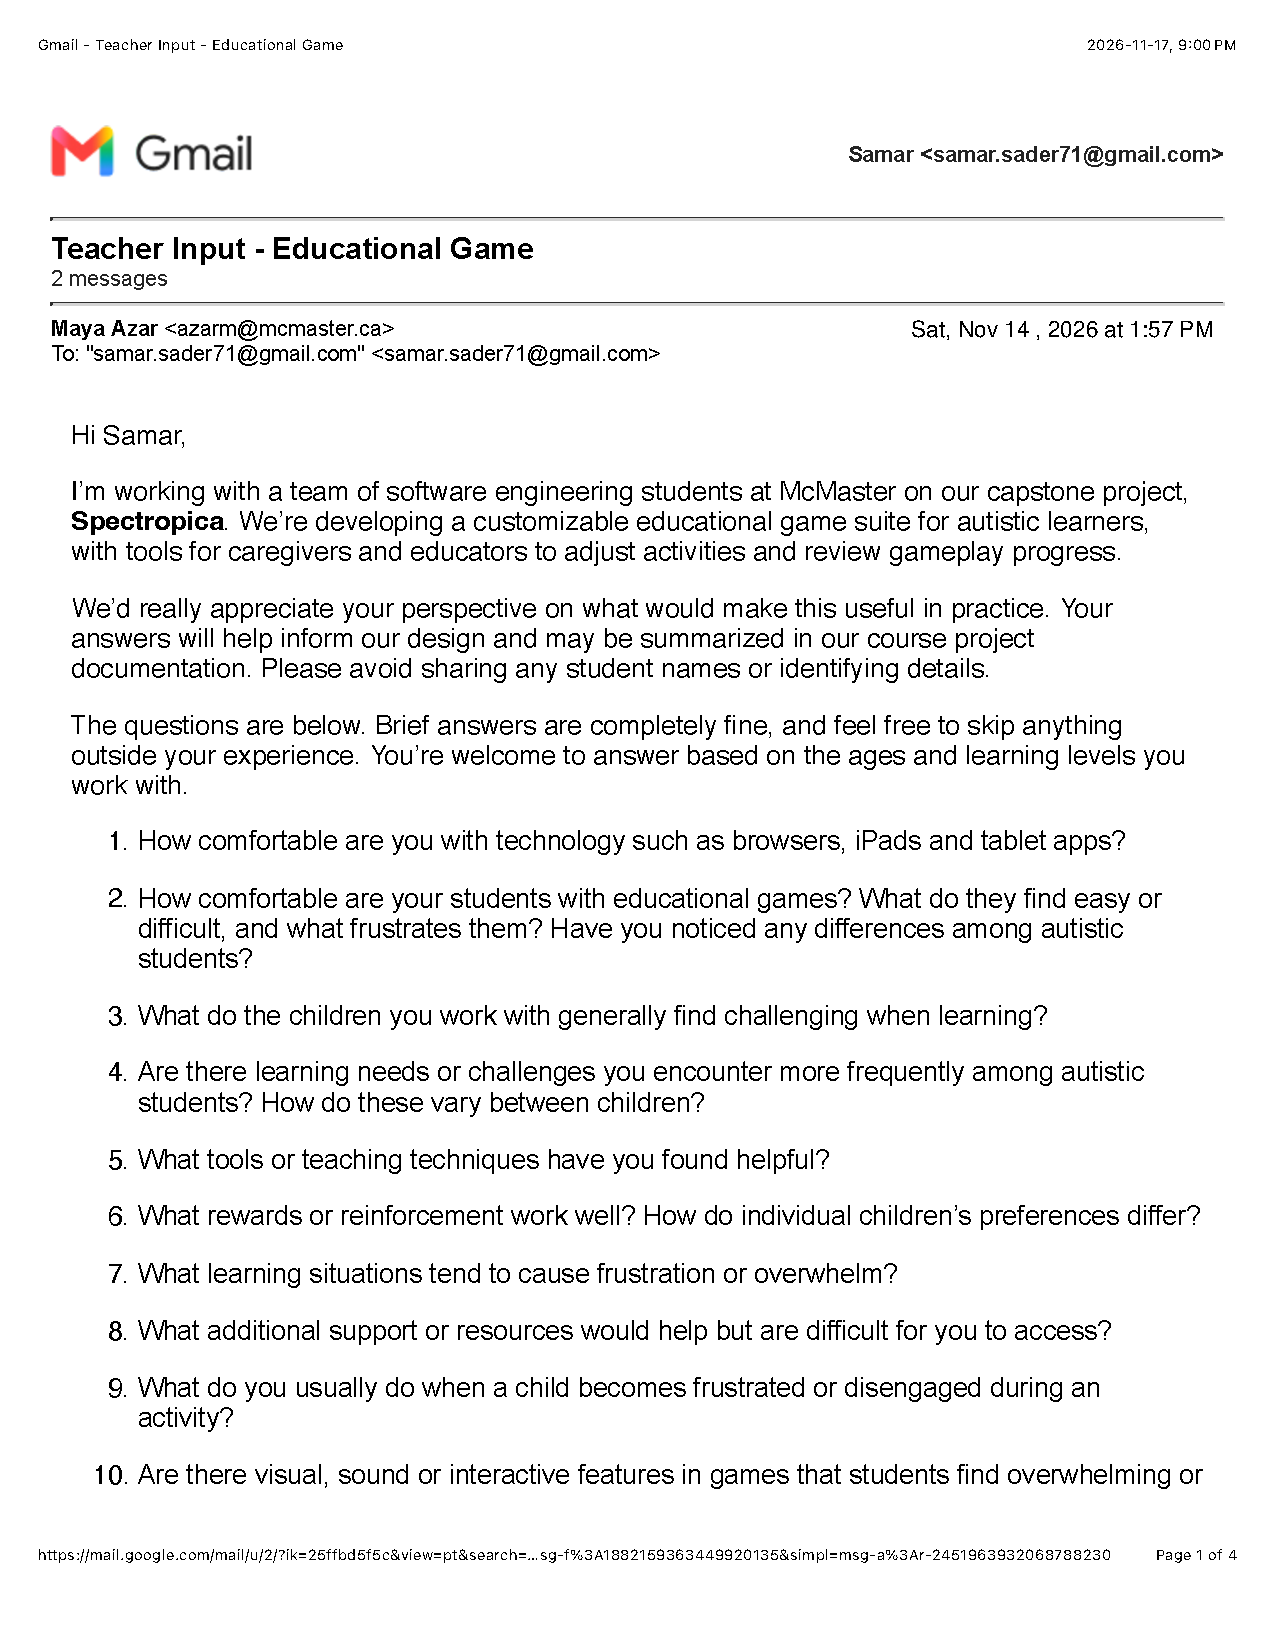
\includepdf[pages=-,scale=0.92,pagecommand={\thispagestyle{plain}}]
  {P1-Email-Exchange.pdf}

\subsection{Educational Assistant Interview (P2)}
\label{app:participant-2}

\noindent\textbf{Collection method:} Interview questionnaire.

\noindent\textbf{Participant:} Educational assistant with an early childhood education background and experience supporting students, including autistic students, across elementary and secondary settings.

The original 21-question response record follows. Question 8 was unanswered,
and Question 7 referred to an earlier response.

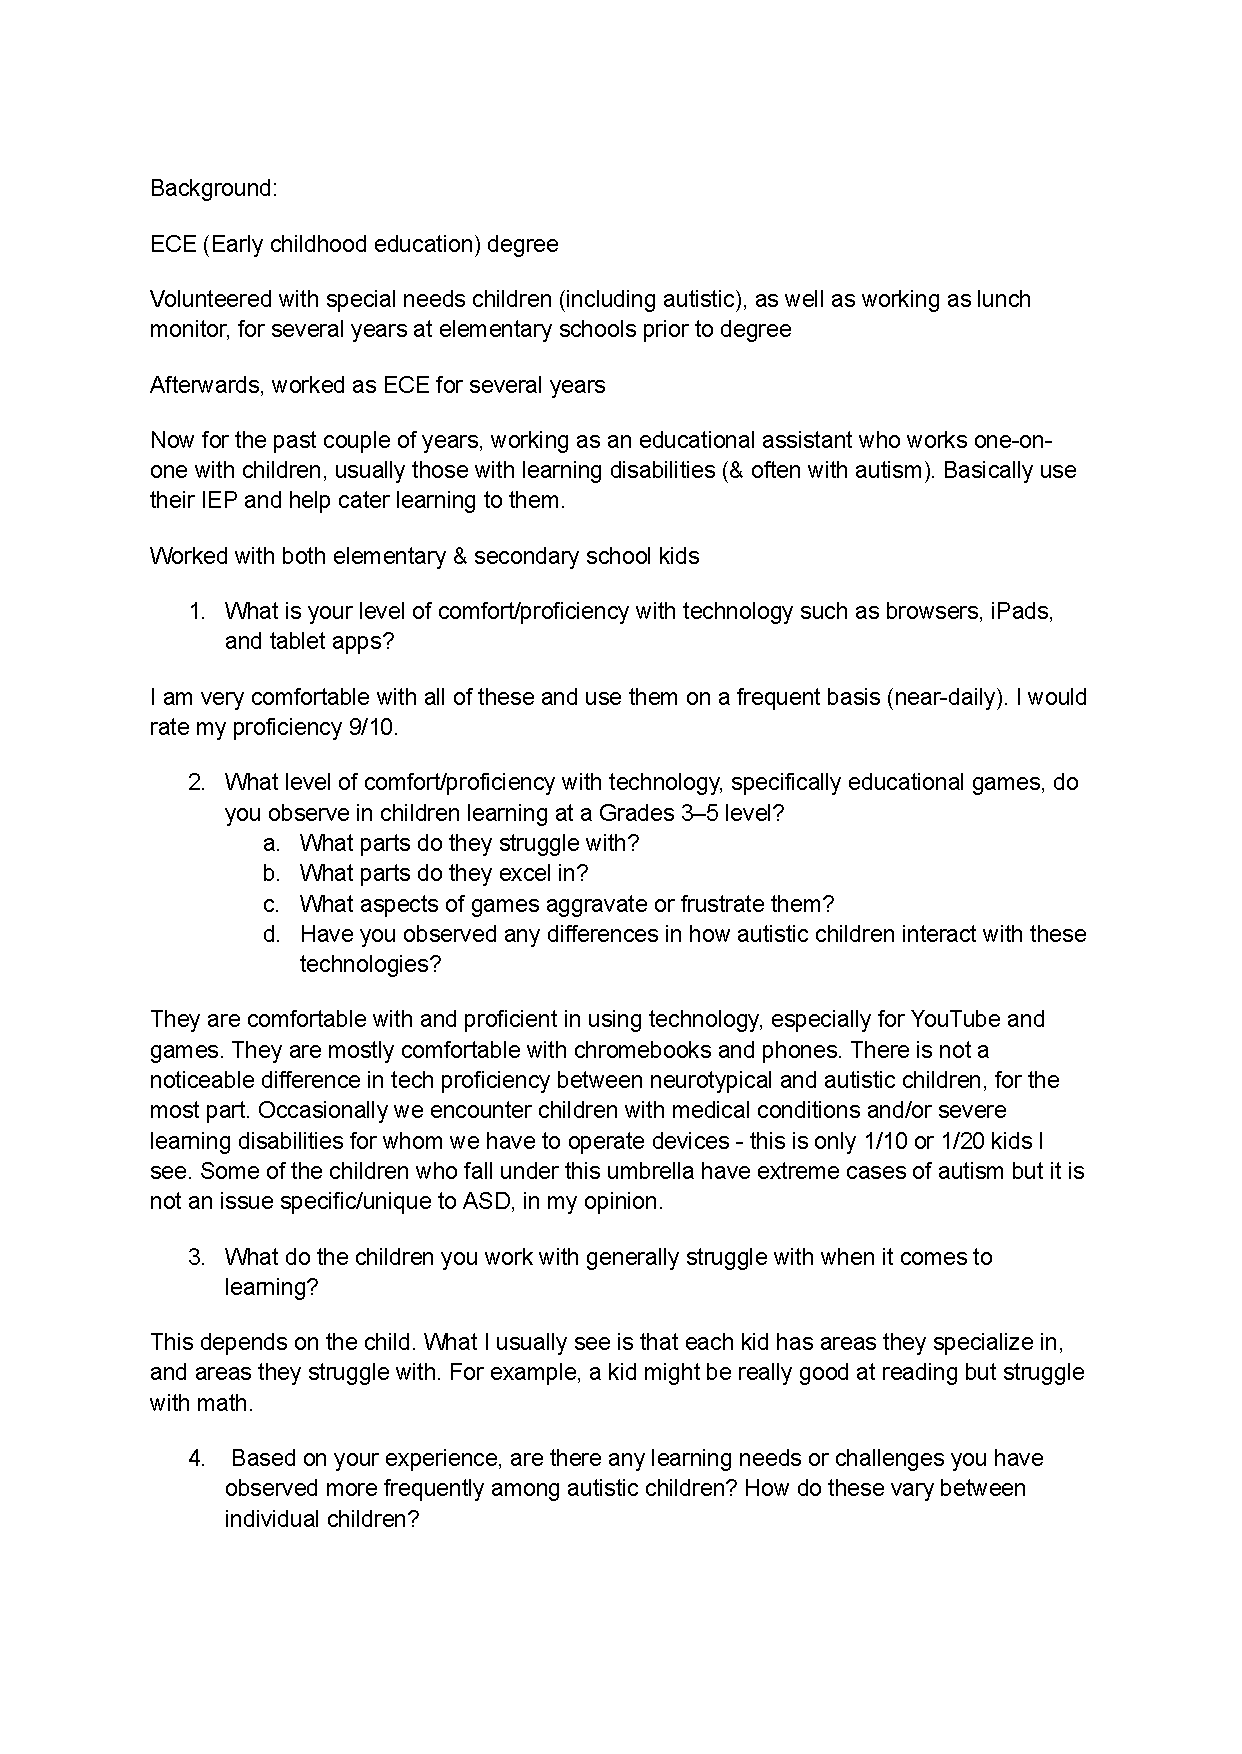
\includepdf[pages=-,scale=0.92,pagecommand={\thispagestyle{plain}}]
  {P2-Educational-Assistant-Transcript.pdf}

\subsection{Developmental Psychology Interview (P3)}
\label{app:participant-3}

\noindent\textbf{Date:} November 2, 2026.

\noindent\textbf{Participant:} Developmental psychology expert and project supervisor.

\noindent\textbf{Source:} Meeting notes rather than a verbatim transcript.

The discussion addressed the intended learner age range, curriculum alignment, CTM customization, sensory controls, reward design, 2D versus 2.5D presentation, and usability testing.

The notes recorded the following considerations:
\begin{itemize}
\item Ontario's curriculum could provide a starting framework for educational activities.
\item A cashier-style activity could focus on reading and arithmetic.
\item CTMs should have meaningful access to game settings.
\item Learners could benefit from controlling stimulation and content.
\item A 2.5D interface could be engaging but might introduce unnecessary distractions.
\item Sound controls, high-contrast problem presentation, and varied rewards should be considered.
\item The team should identify how Spectropica differs meaningfully from existing games.
\end{itemize}

These are summaries of the documented discussion, not verbatim quotations.

\subsection{Care Team Member Interview (P4)}
\label{app:participant-4}

\noindent\textbf{Collection method:} Interview questionnaire.

\noindent\textbf{Participant:} Care Team Member.

\begin{quote}
\sffamily
\noindent\textbf{1. What is your level of comfort/proficiency with technology such as browsers, iPads, and tablet apps?}

\noindent 10/10

\noindent\textbf{2. What level of comfort/proficiency with technology, specifically educational games, do you observe in children learning at a Grades 3–5 level? a. What parts do they struggle with? b. What parts do they excel in? c. What aspects of games aggravate or frustrate them? d. Have you observed any differences in how autistic children interact with these technologies?}

\noindent 7/10 Question 2(a–d) — notes without an attributed speaker a) There are games he deletes because he doesn’t understand them b) Good at typing, good at understanding buttons and icons (typical UI elements) c) Limitation on live count, background music not liked d) Enjoyment of repetition of very specific elements such as music or video, might only play one or 2 games of many

\noindent\textbf{3. What do the children you work with generally struggle with when it comes to learning?}

\noindent Struggling to care about the task, monotone activities (unless they enjoy its specific repetition), learning with others, distracting elements that take away from the learning task

\noindent\textbf{4. Based on your experience, are there any learning needs or challenges you have observed more frequently among autistic children? How do these vary between individual children? 5. What tools or techniques help?}

\noindent significant encouragement, periodic rewards that elicit the same emotional response, befriending them, making clear the time to learn and the time to play freely

\noindent\textbf{6. What types of rewards or reinforcement have you found effective for children generally? Have you noticed differences in how individual autistic children respond?}

\noindent Food especially chocolate and candy, cosmetics, access to play, words of affirmation

\noindent\textbf{7. What circumstances of learning aggravate them?}

\noindent Blunt “do this” instructions, no clear incentive, lack of ‘fun’ elements, visually blocked things (eg. games they can’t play)

\noindent\textbf{8. What is hard to do on your own or outside your control but would help?}

\noindent Sentence construction, reinforcement of learned vocabulary in different contexts, replacing some games that lack educational elements

\noindent\textbf{9. When a child becomes frustrated or disengaged during a learning activity, what strategies do you use to help them?}

\noindent Bringing the energy down (calming) then re-entering the activity, fast-tracking a reward (not often to not associate frustration with rewards), fast-tracking a hint, giving a small break, verbal encouragement, saying it’ll be done soon

\noindent\textbf{10. Are there particular visual, auditory, or interactive features in educational games that children find overwhelming or distracting?}

\noindent If there is too much happening in the background visually, it can distract from the task. Repetitive elements (eg. replaying noise) is good for education and engagement but can definitely be distracting, visually locked stuff is distracting

\noindent\textbf{11. What accommodations or accessibility features have you found most effective when supporting autistic children during digital learning activities?}

\noindent hint or help (?) buttons, replaying the instructions for a task, supporting visual instructions with audio, SFX control

\noindent\textbf{12. What aspects of an educational game would be most valuable to customize, such as difficulty, visuals, sounds, instructions, or activity duration?}

\noindent Duration of activity to tailor to the child’s attention span, wording of hints, reward access

\noindent\textbf{13. How do you measure their progress in learning?}

\noindent Recalling learnt information when asked later, connecting information together (eg. learning counting + fruit vocabulary -> 3 apples), less resistance in learning activities shows willingness to learn (which itself needs to be learnt), better social cues such as not taking something without asking

\noindent\textbf{14. What is hard to track manually but would be helpful to have documented over time?}

\noindent Vocabulary recall, math proficiency, level of engagement, speed of solving

\noindent\textbf{15. What indicators tell you that a child is improving at a particular skill? 16. What information would you want an educational game to record automatically?}

\noindent When difficulties are completed multiple times at a sufficient level, time between instruction and attempt, time between attempts, how many mistakes before correcting, if there are common pitfalls, if there are common successes

\noindent\textbf{17. What educational games or learning tools do you currently use with children, and what features do you find most helpful?}

\noindent Otismo, Cubic Frog, Talking Tom/Angela/Ben

\noindent\textbf{18. When children use educational games, how much assistance do they typically need from an adult? Are there particular tasks they struggle to complete independently?}

\noindent needs help unlocking, needs help adjusting settings, needs help understanding different options to accomplish the same task, needs help in time-based games (eg. must wait before doing X, must finish task in Y time)

\noindent\textbf{19. What would make a progress dashboard easy or difficult for you to interpret?}

\noindent line graphs, bar graphs, contrasting color themes, lots of tooltips, easy to export data

\noindent\textbf{20. What are the biggest limitations of the current games that exist?}

\noindent insufficient customization for stimulation or distraction levels, insufficiently satisfying rewards, poor instructions not explaining well enough, incentive not clear

\noindent\textbf{21. If you were to use an educational game like Spectropica with a child, what improvements or outcomes would make you consider it successful?}

\noindent progressively meeting learning objectives, easy visualization for Care Team, easy sharing of data between Care Team, customizing the settings for different kids or for the same kid when the latter shows discomfort or disengagement from current settings

\end{quote}

\subsection{Parent Interview (P5)}
\label{app:participant-5}

\noindent\textbf{Collection method:} Interview questionnaire.

\noindent\textbf{Participant:} Parent of an autistic child.

\begin{quote}
\sffamily
\noindent\textbf{1. What is your level of comfort/proficiency with technology such as browsers, iPads, and tablet apps?}

\noindent 9/10, easy usage

\noindent\textbf{2. What level of comfort/proficiency with technology, specifically educational games, do you observe in children learning at a Grades 3–5 level? a. What parts do they struggle with? b. What parts do they excel in? c. What aspects of games aggravate or frustrate them? d. Have you observed any differences in how autistic children interact with these technologies?}

\noindent 5/10\par\noindent Question 2(a–d) — notes without an attributed speaker\par\noindent a) There are games he deletes because he doesn’t understand them b) Good at typing, good at understanding buttons and icons (typical UI elements) c) Limitation on live count, background music not liked d) Enjoyment of repetition of very specific elements such as music or video, might only play one or 2 games of many

\noindent\textbf{3. What do the children you work with generally struggle with when it comes to learning?}

\noindent Requires highly simplified learning patterns, super guided, what it means to ‘win’ or ‘lose’ without a physical reward, requires an emotional reward, unliked concepts must be introduced very slowly and via feeding within liked concepts

\noindent\textbf{4. Based on your experience, are there any learning needs or challenges you have observed more frequently among autistic children? How do these vary between individual children? 5. What tools or techniques help?}

\noindent Parent ABA courses

\noindent\textbf{6. What types of rewards or reinforcement have you found effective for children generally? Have you noticed differences in how individual autistic children respond?}

\noindent Food when he was younger, access to fun things when he was older such trampoline or coloring or clay or youtube, even older it was more congratulatory like clapping or dancing or words of affirmation. Enjoyed blowing bubbles and trying to catch them

\noindent\textbf{7. What circumstances of learning aggravate them?}

\noindent Visual or auditory distractors such as people talking or walking, background noises, background furniture

\noindent\textbf{8. What is hard to do on your own or outside your control but would help?}

\noindent More social with similarly aged family (e.g. cousins), waiting in line, teaching cooperation within games (does not understand teamwork)

\noindent\textbf{9. When a child becomes frustrated or disengaged during a learning activity, what strategies do you use to help them?}

\noindent Telling him at a specific time, this activity will end so it will not continue forever. Promise of future rewards or enjoyment such as going out or games

\noindent\textbf{10. Are there particular visual, auditory, or interactive features in educational games that children find overwhelming or distracting?}

\noindent Overwhelming interactive elements are usually cooperation

\noindent\textbf{11. What accommodations or accessibility features have you found most effective when supporting autistic children during digital learning activities?}

\noindent I don’t know

\noindent\textbf{12. What aspects of an educational game would be most valuable to customize, such as difficulty, visuals, sounds, instructions, or activity duration?}

\noindent Different voices for auditory elements, visual themes with a lot of moving parts, slowly rising difficulties

\noindent\textbf{13. How do you measure their progress in learning?}

\noindent When he starts generalizing skills he learnt, such as reusing sentences or words in correct context

\noindent\textbf{14. What is hard to track manually but would be helpful to have documented over time?}

\noindent Vocabulary, hygienic tendencies, social skills (eye contact, please \& thank you), physical skills in swimming for example, willingness to accept change, willingness to cooperate with others

\noindent\textbf{15. What indicators tell you that a child is improving at a particular skill? 16. What information would you want an educational game to record automatically?}

\noindent completing a certain difficulty

\noindent\textbf{17. What educational games or learning tools do you currently use with children, and what features do you find most helpful?}

\noindent Cubic Frog, Proloquo2Go

\noindent\textbf{18. When children use educational games, how much assistance do they typically need from an adult? Are there particular tasks they struggle to complete independently?}

\noindent Cooperation with others, unlocking levels, understanding different ‘weapons’ in toy blast

\noindent\textbf{19. What would make a progress dashboard easy or difficult for you to interpret?}

\noindent divided skill sections, easy to see what level they are at in every skill or game, percentages, options for table, pie charts, different colors, lots of dates (date pickers)

\noindent\textbf{20. What are the biggest limitations of the current games that exist?}

\noindent first level is too difficult, vocabulary too complex for his level, understimulation (not enough moving parts)

\noindent\textbf{21. If you were to use an educational game like Spectropica with a child, what improvements or outcomes would make you consider it successful?}

\noindent helps Care Team to evaluate the mental age of the child, then shows what goals the child should reach and what games would help with it, then checks off the ‘stage’ of a goal when the child has surpassed the level

\end{quote}

\subsection{Source Record}

The report draws on the following material:
\begin{enumerate}
\item Special education teacher email responses.
\item Educational assistant interview questionnaire.
\item Developmental psychology interview notes, November 2, 2026.
\item \emph{Fall CD Interview Questions.pdf}, containing the CTM and parent responses.
\item The team's \href{https://github.com/meena-alomran/game-n-grow/blob/main/docs/CDs/Interviews/Expectations.md}{GitHub Interview Report Expectations}.
\end{enumerate}

\section{Generative AI Use Disclosure}

\subsection{AI Tools Used}

ChatGPT (OpenAI GPT-6) was used to assist with the preparation of the
Stakeholder Interview Report Custom Document (CD).

\subsection{How and Where Used}

ChatGPT was used to assist with organizing and formatting the report based on
the stakeholder interview responses and meeting notes provided by the team.

Specifically, ChatGPT assisted with structuring the appendices, formatting
the interview transcripts, and organizing the list of interview questions in
Section~\ref{sec:interview-questions}.

It was also used to identify connections between stakeholder feedback and
Spectropica's modules in Section~\ref{sec:development-traceability}.

Additionally, ChatGPT assisted with reviewing grammar and clarity throughout
the document and converting the report into \LaTeX{} format.

\subsection{Verification of AI-Generated Content}

The team reviewed the AI-assisted content against the original stakeholder
interview responses and meeting notes to ensure that participant statements
were accurately represented and that no information or quotations were
fabricated.

The connections identified in Section~\ref{sec:development-traceability} were
reviewed against Spectropica's module definitions to ensure consistency with
the system's design.

The \LaTeX{} source code and compiled PDF were inspected to verify the
formatting of the interview transcripts, tables, appendices, and section
organization.

Grammar and clarity suggestions were reviewed to ensure that the original
meaning of the stakeholder responses was preserved.

The team remains responsible for the accuracy, completeness, and consistency
of the final document.

\end{document}
